{\color{ink}\fontsize{18}{21}\selectfont\bfseries BMMC data: increasing the probe count\par}
{\small\color{muted}Experiment results \enspace / \enspace verified 9 October 2026 \hfill 9 of 9 runs completed\par}
\vspace{4pt}
\textbf{Data.} Bone-marrow mononuclear cells (BMMC): all 6,224 cells in each of
the downloaded processed moscot RNA and ATAC files, with no additional cell
subsampling (38,738,176 coupling variables). RNA uses 50 provided PCA coordinates;
ATAC uses 38 provided LSI coordinates, normalized rowwise to unit Euclidean norm.
Within-view Euclidean distances are divided by each matrix's own maximum.
The views are independently reordered; masses are uniform and labels are unused.

\textbf{Design.} Stochastic FraMES with 128, 1,024 or 2,048 random-sign probes per
gradient; three development seeds (710--712), 20,000 updates each, product start
$P_0=ab^\top$, and one Ruche A100 per run. One gradient estimate is formed per
update, with $d_0=\widehat G_0$. All other settings are fixed across probe counts:
\[
 \gamma_k=(k+1)^{-3/4},\qquad
 \rho_k=0.3(k+1)^{-1/2}\ (k\geq1),\qquad
 \mu_k=\frac{0.1}{6224}(k+1)^{-1/4}.
\]
\vspace{-5pt}
\begin{center}
\small\renewcommand{\arraystretch}{1.16}\setlength{\tabcolsep}{11pt}
\begin{tabular}{@{}rrrr@{}}
\toprule
Probes & Final feasible loss $\downarrow$ & Decrease from $P_0$ & Solver minutes\\
\midrule
128 & 0.16060800 & 0.2680\% & 6.28 \\
1,024 & 0.15900026 & 1.2664\% & 15.13 \\
2,048 & 0.15867071 & 1.4710\% & 24.36 \\
\bottomrule
\end{tabular}
\end{center}
\vspace{-5pt}
{\small Medians across three seeds; initial feasible loss $f(P_0)=0.16103965$.
Percentage decreases are computed per seed before taking the median.}

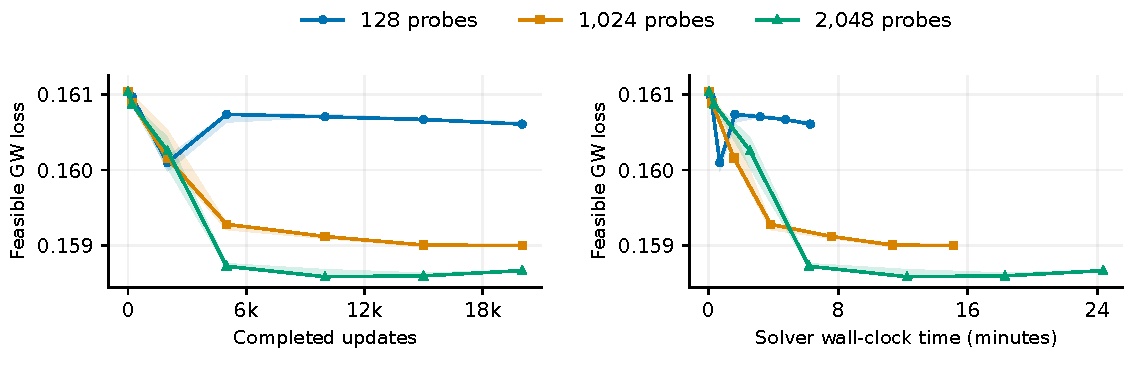
\includegraphics[width=\linewidth]{bmmc_probe_count_status_curves.pdf}
\vspace{-5pt}
{\footnotesize\color{muted}Markers are saved checkpoints; lines are visual guides. Shading shows the three-seed IQR.
The time plot places each common-iteration median loss at its median solver time; it does not interpolate to a common time grid.}

\textbf{Assessment.} Increasing the probe count improves the final feasible
loss at 20,000 updates, but the decrease remains modest and solver cost rises.
The 2,048-probe median reduction is 1.471\%, versus 0.268\% with 128 probes.
These are three random seeds on one fixed processed dataset, not independent
biological replicates. The result does not establish that gradient noise is the
only remaining limitation; biological matching accuracy was not evaluated.

\textbf{Scope.} This comparison changes only the probe count within the stated
configuration. It is not a comparison against another optimization method, nor a
claim that these prefactors are the best ones for BMMC. The processed files used
here are not the entire larger original BMMC collection.

\vfill
{\footnotesize\color{muted}\textbf{Measurement.} Final-iterate loss after transport repair, evaluated in FP64;
initial and intermediate losses use FP32. This is neither a best-checkpoint loss
nor a theorem-selected output. Solver time includes initialization and updates;
it excludes preparation, repairs, loss diagnostics, logging, snapshots and final
FP64 validation. It is not end-to-end elapsed time.\\[3pt]
\textbf{Provenance.} Frozen instance \texttt{bmmc6224}; run source \texttt{8d11e2a};
completed probe-study report SHA256 prefix \texttt{6ce0b0198875649d7}.}
